\begin{frame}
	\frametitle{Detección de Keypoints}
	
	\note{https://youtu.be/ebMyBbkkHWk}
	
	\footnotesize
	Propiedades deseables para SLAM / SfM:
	\begin{itemize}
		\item Alta repetitibilidad
		\item Alta precisión
		\item Robustez
		\item Invarianza (luminosidad, puntos de vista, etc)
		\item Computacionalmente eficientes
		\item Algunos detectores: HARRIS, SIFT, SURF, Shi-Tomasi, FAST, ORB, BRISK
	\end{itemize}

	
	\begin{figure}
		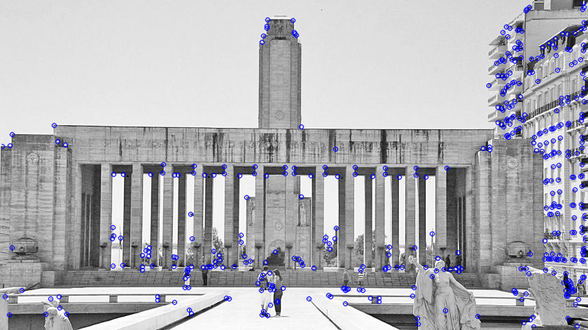
\includegraphics[width=0.5\textwidth]{./images/keypoints_fast}
		\caption{Keypoints FAST}
	\end{figure}

\end{frame}


\begin{frame}
	\frametitle{Matcheo de keypoints}
	\footnotesize
	Propiedades deseables del matcheo de keypoints para SLAM / SfM:
	\begin{itemize}
		\item Alto recall
		\item precisión
		\item Robustez
		\item Computacionalmente eficientes
		\item Posibles enfoques: patches o descriptores
	\end{itemize}
	
	\begin{figure}
		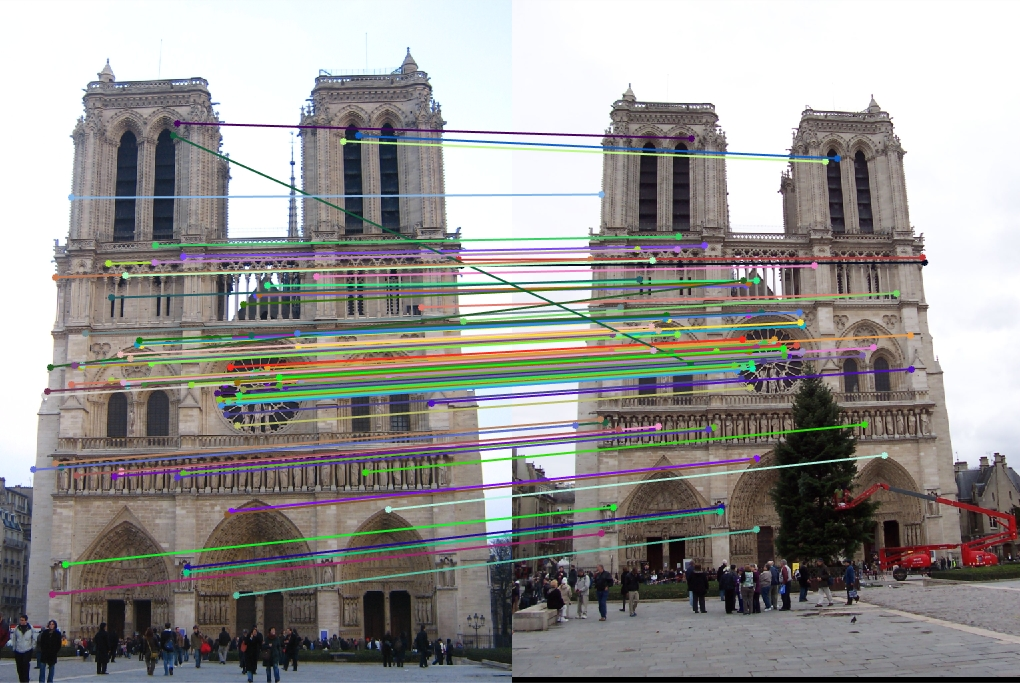
\includegraphics[width=0.4\textwidth]{./images/matching_notredam.jpg}
		\caption{Keypoints Harris + Descriptor SIFT}
	\end{figure}
	\note{Imagen extraida de https://www.cc.gatech.edu/classes/AY2016/cs4476_fall/results/proj2/html/cpolack6/index.html}
\end{frame}

\begin{frame}
	\frametitle{Precision - Recall}
	\footnotesize
	
	\note{https://upload.wikimedia.org/wikipedia/commons/2/26/Precisionrecall.svg}
	
	\begin{figure}
		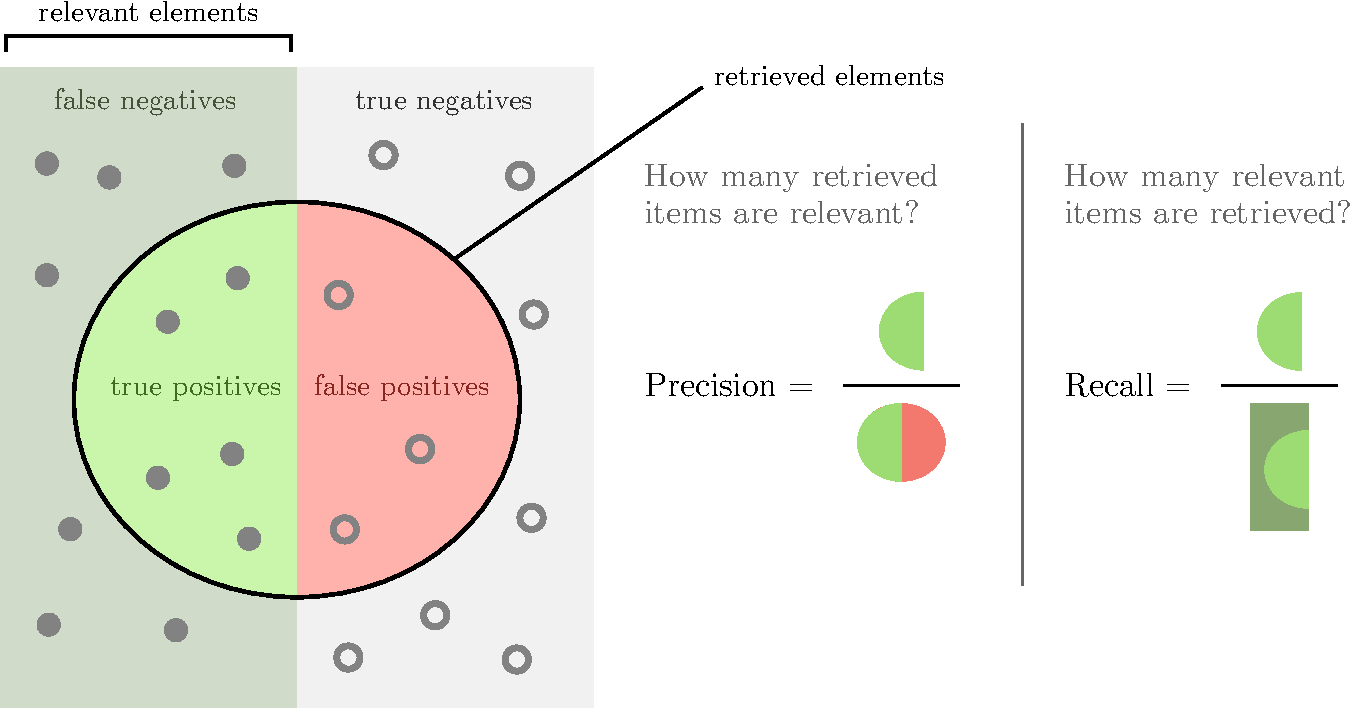
\includegraphics[width=0.25\textwidth]{./images/precision_recall.pdf}
	\end{figure}
\end{frame}

\begin{frame}
	\frametitle{Desciptores de features Locales}
	\footnotesize
	
	Propiedades deseables para SLAM / SfM: distinguibles, robustos, invariantes
	\begin{itemize}
		\item Extraer firmas sobre regiones de la imagen ejemplos:
		\begin{itemize}
			\item Histogramas sobre gradientes de la imagen (SIFT)
			\item Histogramas sobre respuestas Haar-wavelet (SURF)
			\item Patrones binarios (BRIEF, BRISK, FREAK, ORB)
			\item Descriptores basados en aprendizaje
		\end{itemize}
		\item Invariante rotación: Alineado con la orientación dominante de la región local
		\item Invariante a escala: Adaptar la región descripta a la escala de keypoint
	\end{itemize}

	\TODO{agregar imagenes SIFT BRIEF}
	
\end{frame}

\begin{frame}
	\frametitle{Local Features invariantes}
	\footnotesize
	
	\begin{itemize}
		\item Invarianza geométrica: traslación, rotación, escala.
		\item Invarianza fotométrica: brillo, exposición, etc.
	\end{itemize}
	 

\end{frame}

\begin{frame}
	\frametitle{Ventajas de features locales}
	\footnotesize

	\begin{itemize}
	\item Locales: los features al ser locales son robustos a oclusiones
	\item Distintivos: pueden diferenciar un gran conjunto de objetos
	\item Cuantiosos: puede haber cientos o miles en una misma imagen
	\item Eficientes: al discretizar la imagen, se puede obtener tiempo real.
\end{itemize}
	
\end{frame}

\begin{frame}
	\frametitle{Harris}
	\footnotesize
	
	\TODO{Agregar slides de SIFT, HARRIS, FAST y ORB https://youtu.be/ebMyBbkkHWk}
	
\end{frame}

\begin{frame}
	\frametitle{Matcheo de keypoints}
	\footnotesize
	
\end{frame}

\begin{frame}
	\frametitle{RANSAC: Random Sample Consensus}
	\footnotesize
	
	\begin{itemize}
		\item Permite encontrar un modelo que ajusta datos en presencia de ruido y outliers
		\item Separa el conjunto de datos entre inliers y outliers
%		\item Encuentra la mejor partición de puntos en un conjunto de inliers y outliers. Estima un modelo utilizando el conjunto de inliers.
		\item Ejemplo: dado un conjunto de puntos 2D, ajustar una línea 
	\end{itemize}
	
	\begin{figure}
		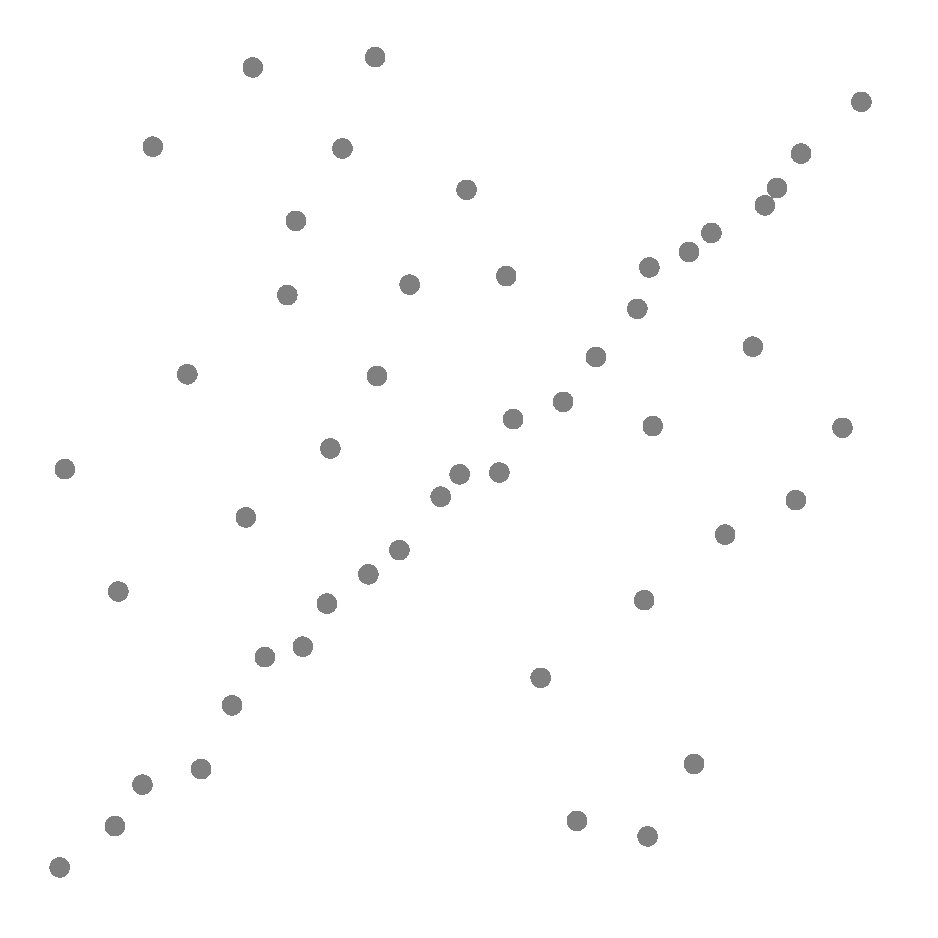
\includegraphics[width=0.5\textwidth]{./images/ransac_points.pdf}
	\end{figure}

	\TODO{hacer imágenes similares a las del vídeo: https://youtu.be/ebMyBbkkHWk}
	
\end{frame}


\begin{frame}
	\frametitle{RANSAC: Random Sample Consensus}
	\footnotesize
	
	\TODO{hacer imágenes similares a las del vídeo: https://youtu.be/ebMyBbkkHWk}
	
	\begin{figure}
		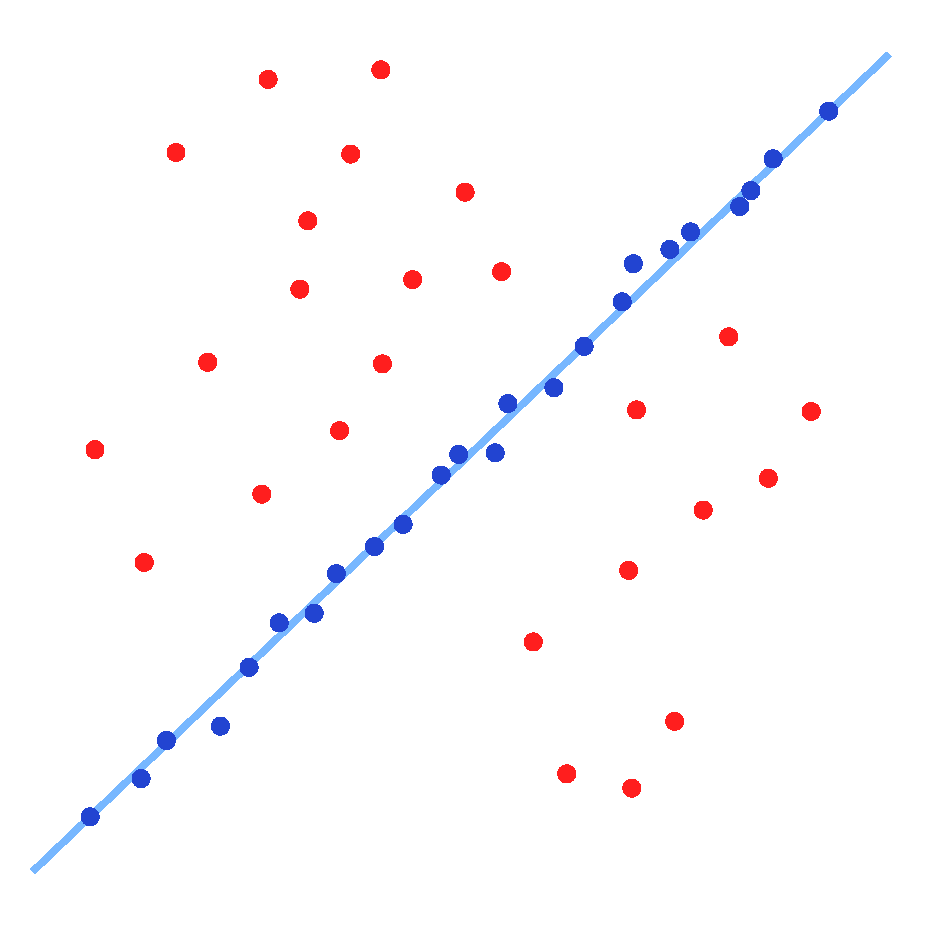
\includegraphics[width=0.5\textwidth]{./images/ransac_fitted_line.pdf}
	\end{figure}
	
\end{frame}
\begin{frame}
	\frametitle{RANSAC: Random Sample Consensus}
	\footnotesize

	\begin{enumerate}
		\item {\bf Samplear} de manera aleatoria el número de puntos requerido para ajustar el modelo.
		\item {\bf Computar} el modelo usando los datos sampleados
		\item {\bf Contar} el número de inliers y quedarse con el modelo que mejor ajusta los datos
		\item Iterar puntos 1-3 hasta que el mejor modelo es hallado
	\end{enumerate}

\end{frame}

\begin{frame}
	\frametitle{RANSAC: Random Sample Consensus}
	\footnotesize
	
	Pero...¿cuantas iteraciones realizar?
	
	\begin{itemize}
		\item Número de puntos sampleados $s$ (número de puntos mínimos requeridos para ajustar el modelo)
		\item Ratio de outliers $e = \dfrac{\# outliers}{\# puntos totales}$
		\item Número de intentos $T$.
		Elegimos $T$, con probabilidad $p$ de éxito (la probabilidad de al menos obtener un muestreo aleatorio libre de outliers en las $T$ iteraciones).
	\end{itemize}
	
	Probabilidad de fallar en una iteración, es decir de no seleccionar todos inliers.
	\begin{equation*}
		1-p = 1 - (1 - e)^{s}
	\end{equation*} 
	\note{(1-e)^s es la probabilidad de seleccionar todos inliers}
	
	
	Probabilidad de fallar en $T$ iteraciones, es decir seleccionar un outlier en todas las iteraciones.
	
	\begin{equation*}
		1-p = (1 - (1 - e)^{s})^{T}
	\end{equation*} 
	despejando $T$,
	\begin{equation*}
		T = \dfrac{\log(1-p)}{\log(1-(1-e)^{s})}
	\end{equation*} 
	
\end{frame}

\begin{frame}
	\frametitle{RANSAC: ventajas y desventajas}
	\footnotesize
	Ventajas:
	\begin{itemize}
		\item Robusto en presencia de outliers
		\item funciona bien para modelos de 1 a 10 parámetros (dependiendo del número de outliers)
		\item Fácil de implementar y entender
	\end{itemize}
	Ventajas:
	\begin{itemize}
		\item El tiempo computacional crece rápido con el porcentaje de outliers y el número de parámetros necesarios para ajustar el modelo
		\item No es bueno para obtener múltiples modelos (e.g. ajustar más de una línea en 2D)
	\end{itemize}
\end{frame}
\begin{frame}
	\frametitle{Geometría Epipolar}
	\footnotesize
	
	\begin{itemize}
		\item La restricción epipolar puede ser computada por medio de puntos 2D en la imagen cuando la pose relative de la cámara es conocida ($\transform{r}{l}$, por ejemplo una cámara estéreo)
		\item El plano epipolar es definido por $\imagePoint_{l}$ y los dos dentros óptico de las cámaras $\cameraCenter_{l}$ y $\cameraCenter_{r}$
		\item La línea epipolar es la intersección del plano epipolar y el plano de la imagen derecha.
		\item La restricción epipolar codifica que $\imagePoint_{r}$ debe estar ubicado sobre la linea epipolar en la imagen derecha.
	\end{itemize}

	\begin{equation*}
		\homoImagePoint_{l}^{\top} \essentialMatrix \homoImagePoint_{r}^{\top} = 0,
	\end{equation*}
	donde $\essentialMatrix = \transform{l}{r}$, y se denomina \emph{Essential Matrix}
	
	La línea epipolar permite que restrinjamos la búsqueda de correspondencias visuales entre dos cámaras.
	
	\TODO{renombrar variables en imágenes}
	
	\begin{figure}
		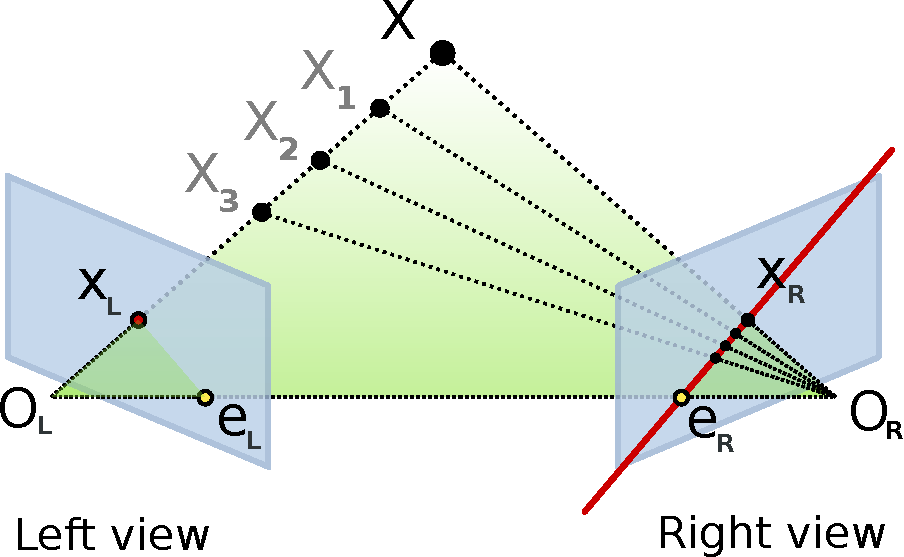
\includegraphics[width=0.4\textwidth]{./images/epipolar_geometry.pdf}
	\end{figure}
	
\end{frame}

\begin{frame}
	\frametitle{Estimación de movimiento}
	\footnotesize
	
	2D-2D
    \begin{columns}
	\begin{column}{0.7\textwidth}
		\begin{itemize}
		\item Error de reproyección:
		\[
		f(\transform{a}{b}, \mapPointsSet)= \sum_{i=1}^{N} \Vert \measurement_{a,i} - \prediction^{\mathrm{s}}(\transform{a}{\worldCoordSystem},\worldPoint_{i}) \Vert^{2} + \Vert \measurement_{b,i} - \prediction^{\mathrm{s}}(\inverse{\transform{a}{b}}\transform{a}{\worldCoordSystem},\worldPoint_{i}) \Vert^{2}
		\]
		\item Algoritmos lineales: 8-point, 5-point
		\end{itemize}
	\end{column}
	\begin{column}{0.3\textwidth}
	    \begin{figure}
			\def\svgwidth{\columnwidth}
			\import{./images/}{tracking_reprojection_error_after.pdf_tex}
		\end{figure}
	\end{column}
\end{columns}

	3D-2D
    \begin{columns}
	\begin{column}{0.7\textwidth}
		\begin{itemize}
			\item Error de reproyección:
			\[
			f(\transform{\worldCoordSystem}{a}, \mapPointsSet)= \sum_{i=1}^{N} \Vert \measurement_{a,i} - \prediction(\inverse{\transform{\worldCoordSystem}{a}},\worldPoint_{i}) \Vert^{2}
			\]
			\item Algoritmos lineales: DLT, PnP
		\end{itemize}
	\end{column}
	\begin{column}{0.3\textwidth}
		\begin{figure}
			\def\svgwidth{\columnwidth}
			\import{./images/}{tracking_reprojection_error_after.pdf_tex}
		\end{figure}
	\end{column}
	\end{columns}
	3D-3D
	\begin{columns}
		\begin{column}{0.7\textwidth}
			\begin{itemize}
				\item Error de reproyección:
				\[
				f(\transform{a}{b})= \sum_{i=1}^{N} \Vert \pointCoord{a}_{i} - \transform{a}{b} \pointCoord{b}_{i} \Vert^{2}
				\]
				\item Algoritmos lineales: Atun, Horn
			\end{itemize}
		\end{column}
		\begin{column}{0.3\textwidth}
			\begin{figure}
				\def\svgwidth{\columnwidth}
				\import{./images/}{tracking_reprojection_error_after.pdf_tex}
			\end{figure}
		\end{column}
	\end{columns}

\end{frame}

\begin{frame}
	\frametitle{Estimación de movimiento 2D-2D}
	\footnotesize
	
	\begin{itemize}
		\item dados los matches 2D-2D $\{(\measurement_{a}, \measurement_{b})_{i}\}$ de puntos 3D desconocidos $\mapPointsSet_{i}$ encontrar el movimiento relativo $\transform{a}{b}$ entre los frames.
		\item Error de reproyección (Bundle Adjustment):
		\[
		f(\transform{a}{b}, \mapPointsSet)= \sum_{i=1}^{N} \Vert \measurement_{a,i} - \prediction^{\mathrm{s}}(\transform{a}{\worldCoordSystem},\worldPoint_{i}) \Vert^{2} + \Vert \measurement_{b,i} - \prediction^{\mathrm{s}}(\inverse{\transform{a}{b}}\transform{a}{\worldCoordSystem},\worldPoint_{i}) \Vert^{2}
		\]
		Se puede optimizar con métodos no lineales pero requieren de una buena semilla inicial. Es no convexo, solución no única (ambigüedadad de escala)
		\item Se puede utilizar un enfoque algebraico basado en geometría epipolar para obtener la transformación relativa (a un factor de escala) sin explicitamente computar la posición de los puntos 3D: algoritmos 8-point y 5-point.
		\item Aplicaciones:
		\begin{itemize}
			\item Filtrar matches con RANSAC
			\item Inicializar una sistemas de SLAM monocular / SfM
		\end{itemize}
	\end{itemize}
\end{frame}

\begin{frame}
	\frametitle{Estimación de movimiento 3D-2D}
	\footnotesize
	
	\begin{itemize}
		\item Dado un conjunto de correspondencias 3D-2D $\{(\worldPoint, \measurement_{a})_{i}\}$ queremos encontrar la pose $\transform{w}{a}$ de la cámara en el mundo.
		\item Error de reproyección:
		\[
		f(\transform{\worldCoordSystem}{a}, \mapPointsSet)= \sum_{i=1}^{N} \Vert \measurement_{a,i} - \prediction(\inverse{\transform{\worldCoordSystem}{a}},\worldPoint_{i}) \Vert^{2}
		\]
		Se puede optimizar con métodos no lineales pero requieren de una buena semilla inicial. Es no convexo, solución no única (ambigüedad de escala)
		\item Este problema es conocido como \emph{Perspective-n-Points} (PnP) y existen diferentes enfoques para resolverlo:
		\begin{itemize}
			\item Direct Linear Transform (DLT)
			\item EPnP
			\item OPnP
		\end{itemize}
		\item Aplicaciones:
		\begin{itemize}
			\item Localización de una cámara dado un mapa de puntos (tracking)
		\end{itemize}
	\end{itemize}
	
\end{frame}

\begin{frame}
	\frametitle{Estimación de movimiento 3D-3D}
	\footnotesize
	
	\begin{itemize}
		\item Dado un conjunto de correspondencias 3D-2D $\{(\worldPoint, \measurement_{a})_{i}\}$ queremos encontrar la pose $\transform{w}{a}$ de la cámara en el mundo.
		\item Error de reproyección:
		\[
		f(\transform{\worldCoordSystem}{a}, \mapPointsSet)= \sum_{i=1}^{N} \Vert \measurement_{a,i} - \prediction(\inverse{\transform{\worldCoordSystem}{a}},\worldPoint_{i}) \Vert^{2}
		\]
		Se puede optimizar con métodos no lineales pero requieren de una buena semilla inicial. Es no convexo, solución no única (ambigüedad de escala)
		\item Este problema es conocido como \emph{Perspective-n-Points} (PnP) y existen diferentes enfoques para resolverlo:
		\begin{itemize}
			\item Direct Linear Transform (DLT)
			\item EPnP
			\item OPnP
		\end{itemize}
		\item Aplicaciones:
		\begin{itemize}
			\item Localización de una cámara dado un mapa de puntos (tracking)
		\end{itemize}
	\end{itemize}
	
	
\end{frame}

\begin{frame}
	\frametitle{Estimación de movimiento 2D-2D}
	\footnotesize
	
\end{frame}

